\documentclass[a4paper,12pt]{extarticle}
\usepackage[utf8]{inputenc}
\usepackage[german]{babel}
\usepackage{amsmath}
\usepackage{amsthm}
\usepackage{amsfonts}
\usepackage{amssymb}
\usepackage{graphicx}
\usepackage{units}
\usepackage{wrapfig}
\usepackage{float}
\usepackage{tikz}
\usepackage{tkz-euclide}
\usetkzobj{all}
\usetikzlibrary{arrows.meta}
\usepackage{multicol}
\usepackage{caption}
\usepackage{verbatim}
\usepackage{hyperref}
\usepackage[european]{circuitikz}
\usepackage{adjustbox}
\usetikzlibrary{shapes.geometric}

\newenvironment{Figure}
  {\par\medskip\noindent\minipage{\linewidth}}
  {\endminipage\par\medskip}


\usepackage[left=2.5cm,right=2.5cm,top=1.8cm,bottom=2cm]{geometry}

\usepackage{pgfplots}
\usepackage{titlesec}

\titleformat*{\section}{\Large \bfseries \sffamily}
\titleformat*{\subsection}{\large \sffamily}


%\date{Abgabe am 12.09.2016}


\newtheoremstyle{problemstyle}  % <name>
        {3pt}                                               % <space above>
        {3pt}                                               % <space below>
        {\normalfont}                               % <body font>
        {}                                                  % <indent amount}
        {\sffamily \bfseries}                 % <theorem head font>
        {\normalfont\bfseries\\}         % <punctuation after theorem head>
        {.5em}                                          % <space after theorem head>
        {}                                                  % <theorem head spec (can be left empty, meaning `normal')>
\theoremstyle{problemstyle}

\newtheorem{problem}{Aufgabe}




\begin{document}

\pagenumbering{gobble}

\begin{multicols}{2}
\parbox{2.5cm}{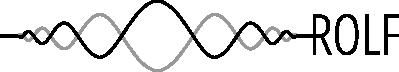
\includegraphics[width=2.5cm]{../task/images/logo_scaled.pdf}}
\parbox{4.5cm}{\centering{\Large \textsf{Notizen zum Seminar Thermodynamik}\\{\small Maximilian Marienhagen\\\url{pankratius.github.io/rolf}}}}
\section*{Temperatur}
\begin{itemize}
\item Maß für mittlere kin. Energie der Teilchen
\item Einheit Kelvin
\item absoluter Nullpunkt bei $0K$
\end{itemize}
\section*{Ausdehnung bei Temperaturänderungen}
\begin{itemize}
\item $\Delta l = \alpha l \Delta T$
\item $\Delta A = \beta A \Delta T, \beta = 2 \alpha$
\item $\Delta V = \gamma V \Delta T, \gamma = 3 \alpha$
\end{itemize}
\section*{Wärme}
\begin{itemize}

\item Def. als Energie, die zwischen thermodynamischen Systemen übertragen wird\\
\item $Q = mc \Delta T$\\
\item Aggregatzustandsänderungen (auch im $T-Q-$Diagramm) $Q \sim m $
\end{itemize}
\section*{Wärmeübertragung}
\begin{itemize}
\item Konvektion
\item Wärmeleitung $P = \lambda\frac{A}{d} \Delta T$
\item Wärmestrahlung
\begin{itemize}
\item Stefan-Boltzmannsches Strahlungsgesetz: $P = \epsilon \sigma A T^4$
\item Kirchhoffsches Strahlungsgesetz: Emissionsgrad $\epsilon$ = Absorptionsgrad $\alpha$
\item Schwarze Körper: $\epsilon = \alpha = 1$
\end{itemize}
\end{itemize}
\begin{problem}
Der Draht einer 100W-Glühbirne ist 10cm lang und hat einen Durchmesser von 0,3mm. Welche Betriebstemperatur hat er?
\end{problem}
\section*{Modell ideales Gas}
\begin{itemize}
\item Teilchen des Gases identische Massepunkte
\item ausschließlich elastische Stöße miteinander und mit Gefäßwänden
\item keine Kräfte
\item Energie auf Freiheitsgrade gleichverteilt
\end{itemize}
\section*{Zustandsänderungen}
\begin{align*}
pv &= nRT & W + Q &= \Delta U \\
U &= \frac{f}{2}nRT & W &= -\int p dV
\end{align*}
\begin{itemize}
\item isochor: $V=konst. \implies W=0$
\item isobar: $p=konst. \implies W = -p\Delta V$
\item isotherm: $T=konst.$
\item adiabatisch: $Q = 0 \implies W = \Delta U$ \\
$pV^\kappa = konst.$ mit $\kappa = \frac{f+2}{f}$
\end{itemize}
\section*{Kreisprozess}
\begin{itemize}
\item periodische Folge von Zustandsänderungen
\item Betrag der Arbeit ist eingeschlossene Fläche im $p-V-$Diagramm
\item für Wärmekraftmaschine: $\eta = \frac{|W|}{Q_{zu}} \leq \frac{T_H-T_K}{T_H}$
\item Durchlaufrichtung beachten!
\end{itemize}
\begin{problem}
Gegeben sei ein rechteckiger Kreisprozess im $p-V-$Diagramm, wobei die Kanten parallel zu den Achsen sind. Finde den Wirkungsgrad
\end{problem}
\end{multicols}
\end{document}